\chapter{Introduction}
\label{chapter:Introduction}

Elementary particle physics is the field of physics that describes the elementary particles and their interactions. The theoretical model denoted by the Standard Model (SM) was created about 50 years ago and is a very successful theory. All its predictions have been confirmed experimentally, including the discovery of the Higgs boson in 2012 at CERN. But theorists believe that there are phenomena predicted by theories beyond the SM that may be discovered at CERN in the next decade, in the future data taking runs, Run-3 Run-4 and Run-5, at the Large Hadron Collider (LHC). There are four major experiments, two of which have general-purpose detectors: ATLAS and CMS. These experiments hope to discover new phenomena like supersymmetry and dark matter. These detectors are huge digital cameras in three dimensions (3D) made of three different layers. Inner detectors reconstruct tracks of charged particles and measure their momenta via ionization energy. Calorimeters measure the total energy of both charged and neutral particles in a destructive process. The final layer is the muon detector, which measures muons tracks as minimum ionization particles.

\ \\The LHC collides bunches of protons. The number of proton-pair collisions per bunch crossing (denoted by the pileup $\mu$) increases steadily every year, to maximise the probability to observe rare processes. Higher $\mu$ values indicate busier collision events and this makes it harder to reconstruct the particles. The latest value of $\mu$ in Run-2 ended in 2018 is about 36. In Run-4 a value of 200 is expected. The potential combinatorics of the events exceeds the available computing power, even with an increased budget. The solution is to reconstruct tracks via new machine learning techniques. This is the problem addressed in this thesis. A public simulated dataset for a general-purpose detector at $\mu$=200 produced for the TrackML Challenge is analyzed in this project. Two key techniques used are a deep neural network and an approximate nearest neighbour technique.

\ \\Sections~\ref{sec:StandardModel} and~\ref{sec:SMLimitations} describe the Standard Model and its limitations. Section~\ref{sec:ExperimentalSetup} describes the experimental setup, and Section~\ref{sec:ProtonCollisions} describes the proton collisions, and Section~\ref{sec:Tracking} describes the tracking reconstruction.

\section{Standard Model}
\label{sec:StandardModel}

The Standard Model is a theory that describes the elementary particle (fermions and bosons) and their interactions via three fundamental forces. The SM elementary particles are illustrated in Figure~\ref{fig:SMParticles} and are described in more detail below.

\begin{figure}[!htb]
  \centering
  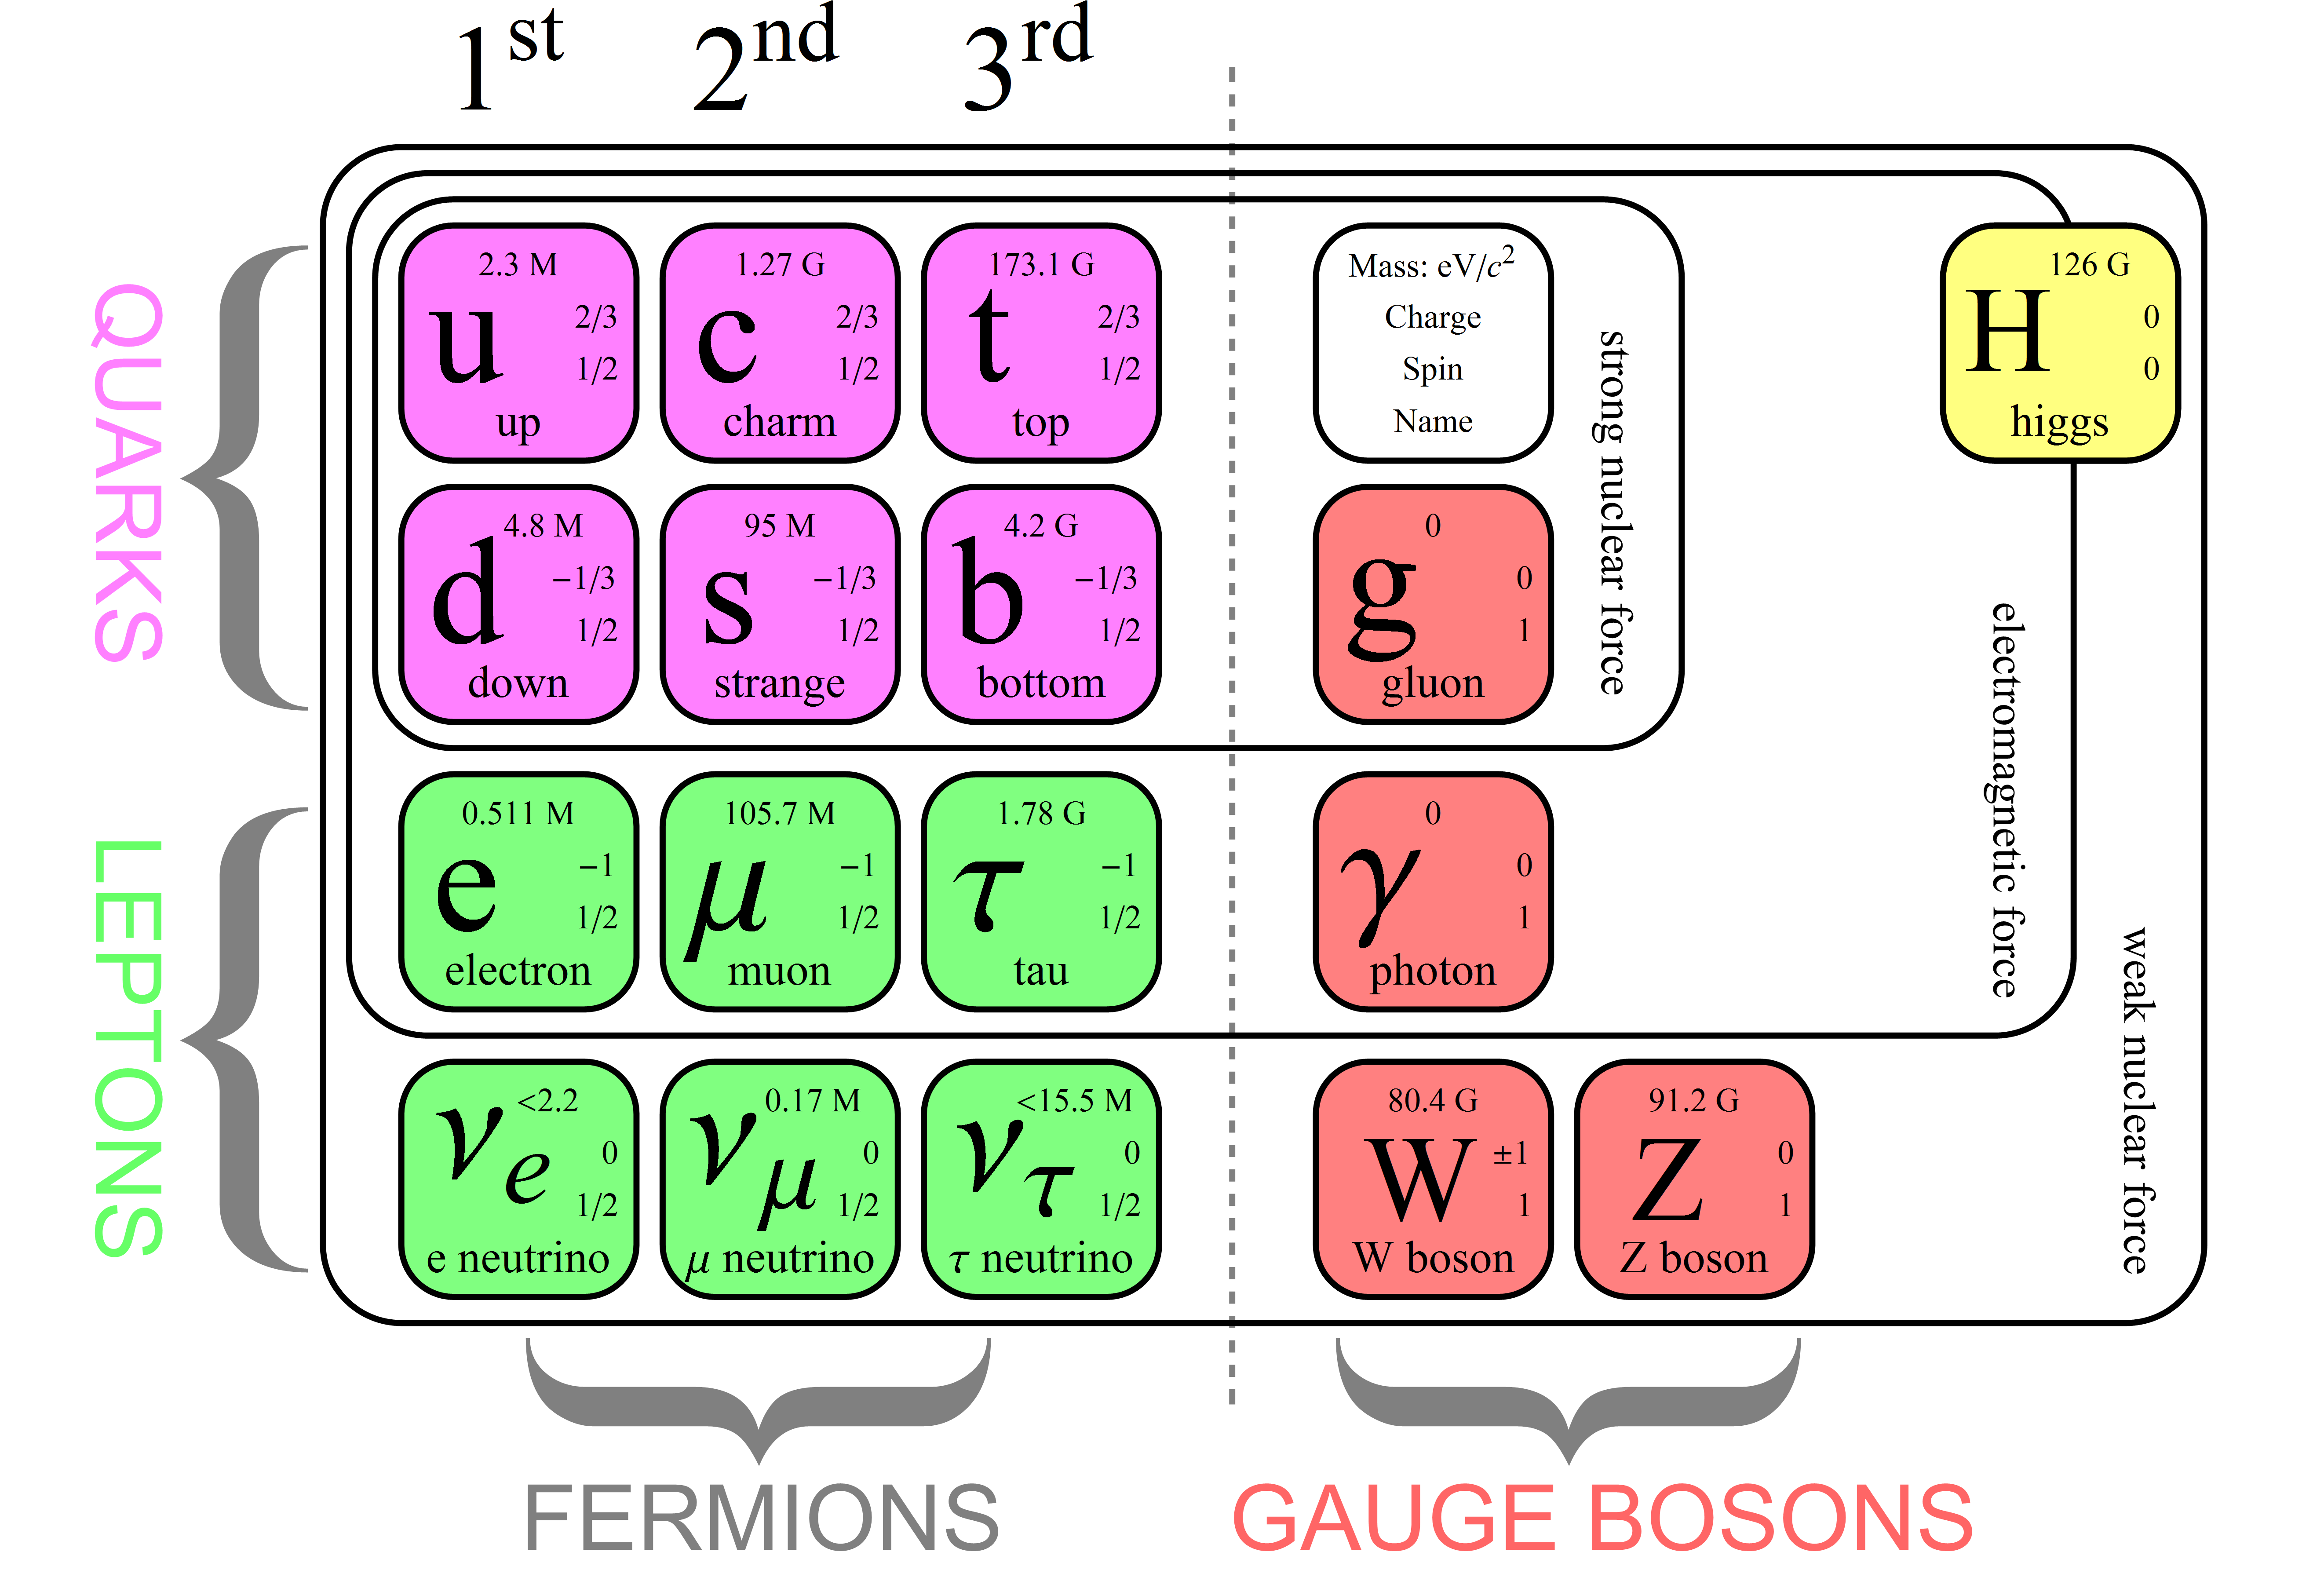
\includegraphics[width=0.98\textwidth]{./plots/SM.png}
  \caption{Elementary particles of the Standard Model}
  \label{fig:SMParticles}
\end{figure}

\ \\There are 12 fermions representing the constituents of matter. They have a semi-integer spin ($1/2$) and they are divided into two categories: quarks and leptons. The quarks have fractional electric charges and form baryons and mesons. The six quarks are up ($u\,^{+2/3}$), down ($d\,^{-1/3}$), charm ($c\,^{+2/3}$), strange ($s\,^{-1/3}$), top ($t\,^{+2/3}$), and bottom ($b\,^{-1/3}$). The three electrically-charged leptons have a negative charge: the electron ($e\,^{-}$), the muon ($\mu\,^{-}$), and the tau lepton ($\tau\,^{-}$). These have corresponding neutrally-charged leptons caled neutrinos ($\nu_e\,^0$, $\nu_\mu\,^0$, $\nu_\tau\,^0$). Together these particles form matter. For each matter particle there is an anti-matter particle that has an opposite electric charge. 

\ \\Fermions interact with each other via the exchange of elementary particles called bosons. Bosons are carriers of the elementary forces and have integer spin ($1$). There are eight type of gluons ($g$) that carry the strong force. The photon ($\gamma$) is responsible for the electromagnetic force. The \Wplus, \Wminus~and the \Zzero~bosons carry the weak force. 

\ \\There is also another type of boson, a scalar elementary particle of spin zero (0), called the Higgs boson. The Higgs boson is the latest elementary particle of the Standard Model discovered in 2012, by the ATLAS and CMS collaborations at CERN. It is predicted by the mechanism explaining how the elementary particles acquire mass.

\section{Limitations of the Standard Model}
\label{sec:SMLimitations}

Although all particles predicted by the Standard Model have been discovered, there are phenomena not yet explained by the SM. 

\ \\The matter-antimatter asymmetry is not yet understood. It is believed in the Big Bang equal quantities of matter and antimatter were produced. But the observable Universe seems to consist of matter only.

\ \\The matter-energy content of the Universe consists of only 5\% of regular baryonic matter. About 25\% is represented by dark matter, an unknown form of matter that interacts only very weakly with regular matter. It is thought this matter is key to the evolution of the Universe.

%\ \\The unification of known fundamental forces is not yet complete. The Standard Model is made of two theories put side by side: the electroweak theory and the quantum chromodynamics, which explains the strong interaction. But these two forces have not yet been unified. Such a unification is thought to happen at energies much larger than those available at the LHC. Such a theory would be called the Grand Unified Theory (GUT). If such a theory were combined further with the gravitational theory at energies close to the Big Bang, the theory of everything (TOE) would emerge.

%\ \\There are three generations of elementary particles. It is not clear why there are exactly three. Particles of each generation are more massive than the previous, but the exact mass values are not yet predicted from first principles. The Higgs mechanism explains how a particle can acquire mass by interacting with the Higgs boson proportional to its mass, but does not predict what the mass is. 

\ \\Overall, it is believed that the Standard Model is in fact only a low-energy approximation of a higher-energy theory. New particles and interactions are predicted by a variety of models of physics beyond the Standard Model (BSM). Such models have already been ruled out by current searches at CERN. The search for new physics will continue in Run-3, Run-4 and Run-5 at the LHC.

\section{Experimental Setup}
\label{sec:ExperimentalSetup}

At the moment the Large Hadron Collider (LHC), which is situated at CERN, is the most powerful proton-proton collider in the world. After the Tevatron and the Large Electron-Positron Collider (LEP) era, a new machine was needed for new discoveries in particle physics. The LHC was designed to achieve a centre-of-mass energy $\sqrt{s}=14\,\TeV$. Two of the biggest goals of the LHC are to study and test the SM, as well as to search for new physics BSM. The LHC accelerator complex is illustrated in Figure~\ref{fig:LHC}.

\begin{figure}[!htb]
  \centering
  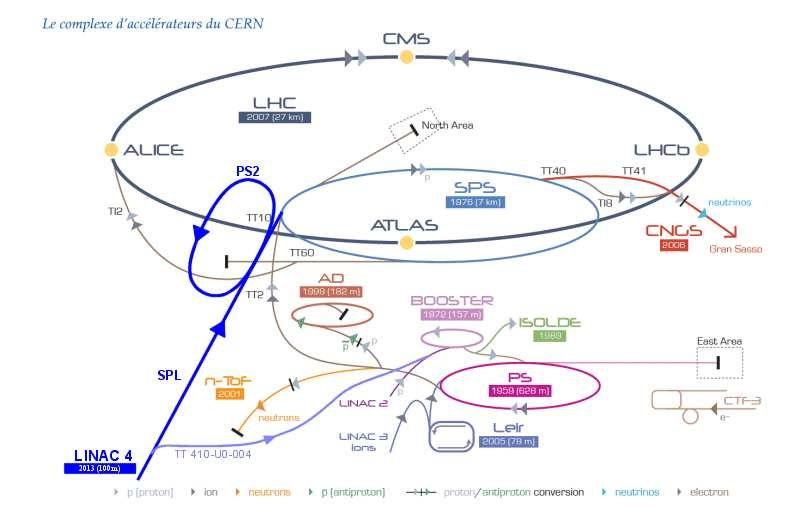
\includegraphics[width=0.5\textwidth]{plots/LHC.png} 
  \caption{LHC Accelerator Complex}
  \label{fig:LHC}
\end{figure}

\ \\This project is affiliated to the international collaboration of the A Toroidal LHC ApparatuS (ATLAS)~\cite{ATLAS}\cite{ATLASUrl}. ATLAS is the largest of several detectors at the LHC. ATLAS is one of two general-purpose particle physics detectors at the LHC, the other being CMS. The two collaborations of ATLAS and CMS perform similar research programs. New discoveries must be observed by both detectors to be believed as true. 

\ \\ATLAS is a cylindrical detector around the colliding proton beams. It is formed of four main subdetectors. The closest to the beam is the inner detector (ID). The ID measures the momentum vector of charged particles which ionise the gas inside the detector. An electric current is measured, giving the position of the particle in the detector, also called a \emph{hit}. A collection of hits forms a \emph{track}. The next detectors the particle encounters are two types of calorimeters, which measure the energy of the particle in a destructive way. The calorimeter is formed of two parts. First there is the electromagnetic calorimeter (EMCal), which measures the energy of electrons, positrons and photons. Then the hadronic calorimeter (HadCal), which measures the energy of hadrons, which originate from quarks and gluons. Several hadrons travelling together, after having originated in the same particle, are called \emph{jets}. Muons deposit very little energy in the calorimeters, being minimum ionising particles. The fourth subdetector detects energy depositions of muons and thus measures their momenta. These subdetectors of ATLAS are illustrated in Figure~\ref{fig:ATLAS}.

\begin{figure}[!htb]
  \centering
  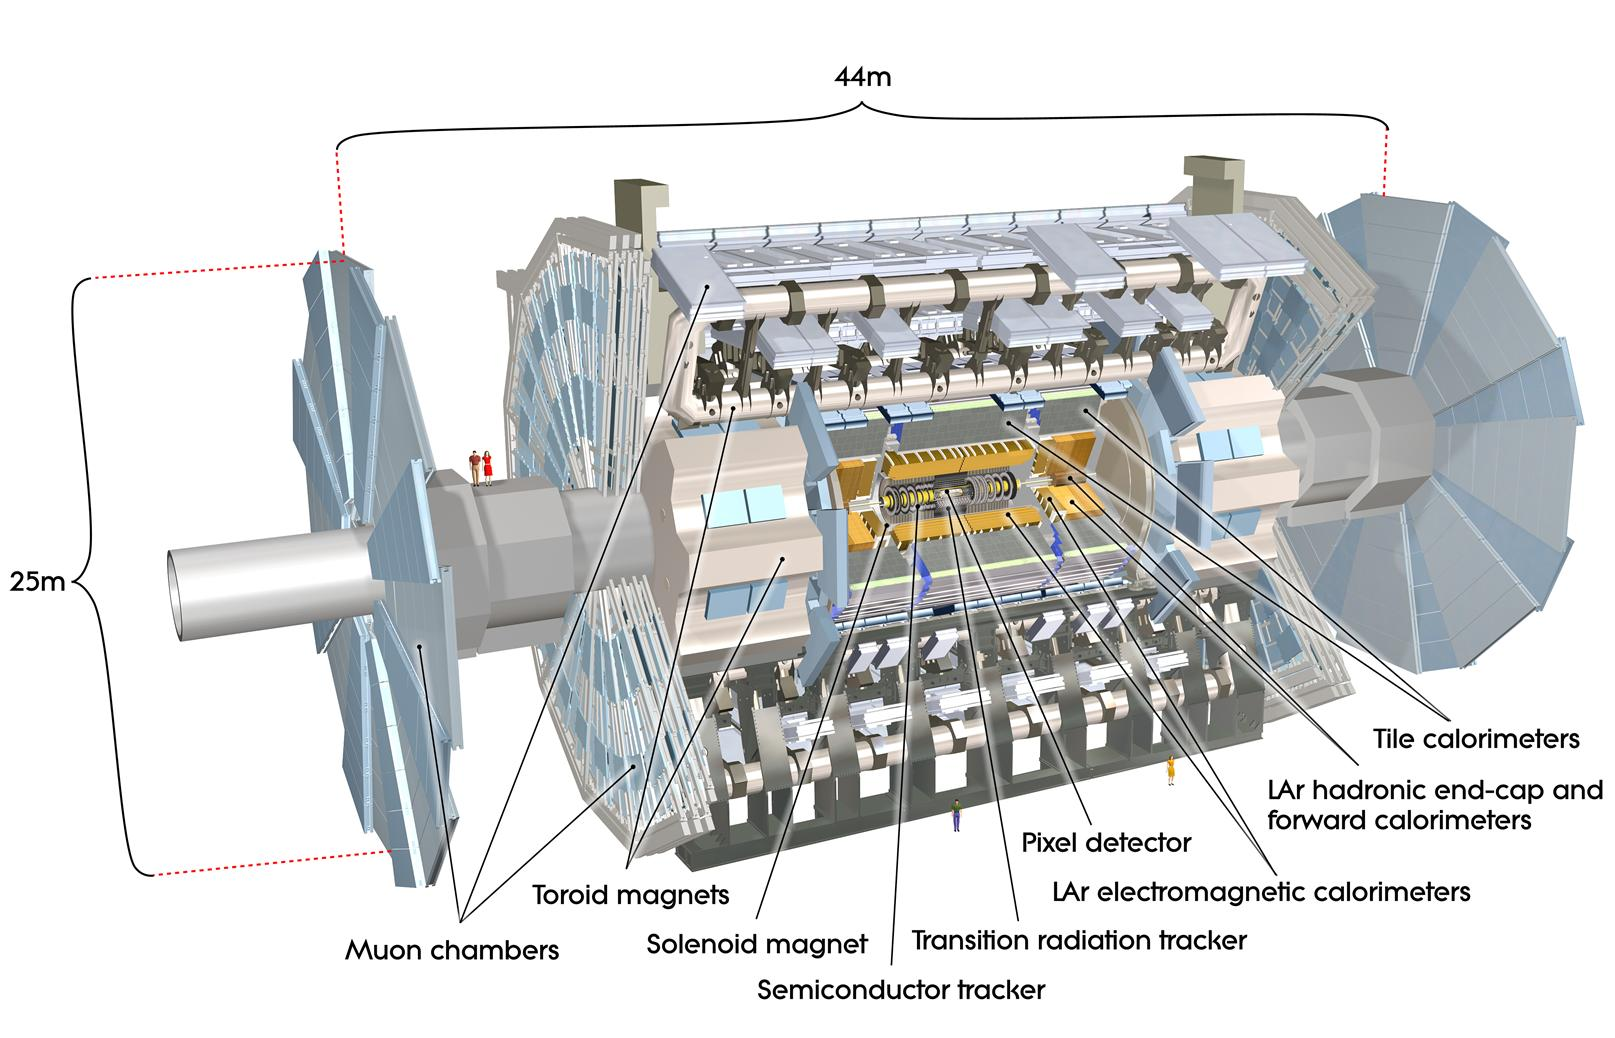
\includegraphics[width=0.5\textwidth]{plots/ATLAS.jpg} 
  \caption{ATLAS detector and its sub-detectors}
  \label{fig:ATLAS}
\end{figure}

\section{Proton Collisions}
\label{sec:ProtonCollisions}

The LHC collides proton beams head-on. The beam is not continuous. Instead, the protons are grouped into up to 2808 bunches. Each bunch contains approximately 115 billion protons. Proton bunches collide every 25 nanoseconds (ns), at a bunch collision rate of 40 MHz. The number of proton collisions during a bunch crossing is called \emph{pile-up} and is denoted by $\mu$. The data from the proton collisions from one bunch crossing are recorded together by the detector, called an an \emph{event}. Usually only one of the collisions produces a rare interesting particle, such as a top quark, a W, Z, or Higgs boson, or BSM particles like supersymmetric candidates or dark matter. The remaining collisions represent a background for the rare one. The rare collision is called \emph{hard scatter} (HS) and the rest of the collisions are called \emph{pile-up} collisions (PU). Event reconstruction in general and charged-particle track reconstruction in particular becomes \emph{harder} with increasing $\mu$. 

\ \\Yet increasing $\mu$ is exactly the strategy employed at the LHC for Run-1 and Run-2, in order to increase the collision luminosity and thus the probability to produce rare particles. The $\mu$ average values during Run-2 were about 13, 25, 38, 36 in 2015, 2016, 2017 and 2018, respectively, as seen in Figure~\ref{fig:LHCPileup}~\cite{ATLASPileup}. In Run-3, Run-4 and Run-5, the aim is to increase the pile-up even further to $\mu=200$.

\begin{figure}[!htb]
  \centering
  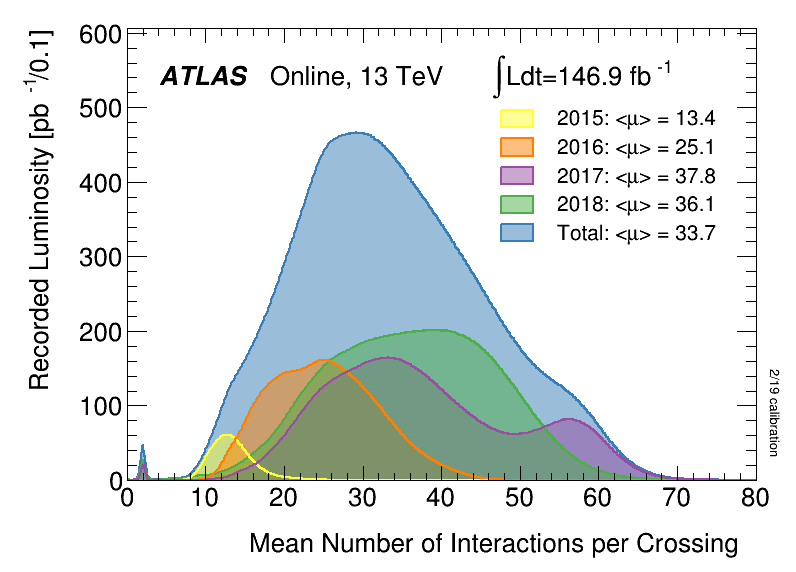
\includegraphics[width=0.5\textwidth]{plots/ATLAS_mu_2015_2018.png} 
  \caption{LHC pile-up ($\mu$) increase during Run-2~\cite{ATLASPileup}}
  \label{fig:LHCPileup}
\end{figure}

\section{Tracking}
\label{sec:Tracking}

A group of hits reconstructed in the inner detector (ID) and belonging to the same particle is called a \emph{track}. Reconstructing particle tracks is called \emph{tracking}. Tracks are produced only by charged particles that ionise the gas in the ID. The ID is held in a magnetic field, so that the trajectories of positively and negatively charged particles curve in opposite directions. The radius of the curvature allows measurement of the particle momentum. Neutral particles, such as photons, neutrinos, and neutral hadrons, do not produce tracks. Because of the magnetic field, tracks are geometric helices pointing approximately to the origin of the primary proton-proton interaction. Reconstructing one track from hits is illustrated in Figure~\ref{fig:FromHitsToTracks}. Reconstructed hits and tracks for an entire collision event are overlaid in Figure~\ref{fig:FromHitsToTracks2}, using simulated data for a general-purpose particle detector. The data is from the TrackML Challenge dataset used in this project. 

\begin{figure}[!htb]
\centering
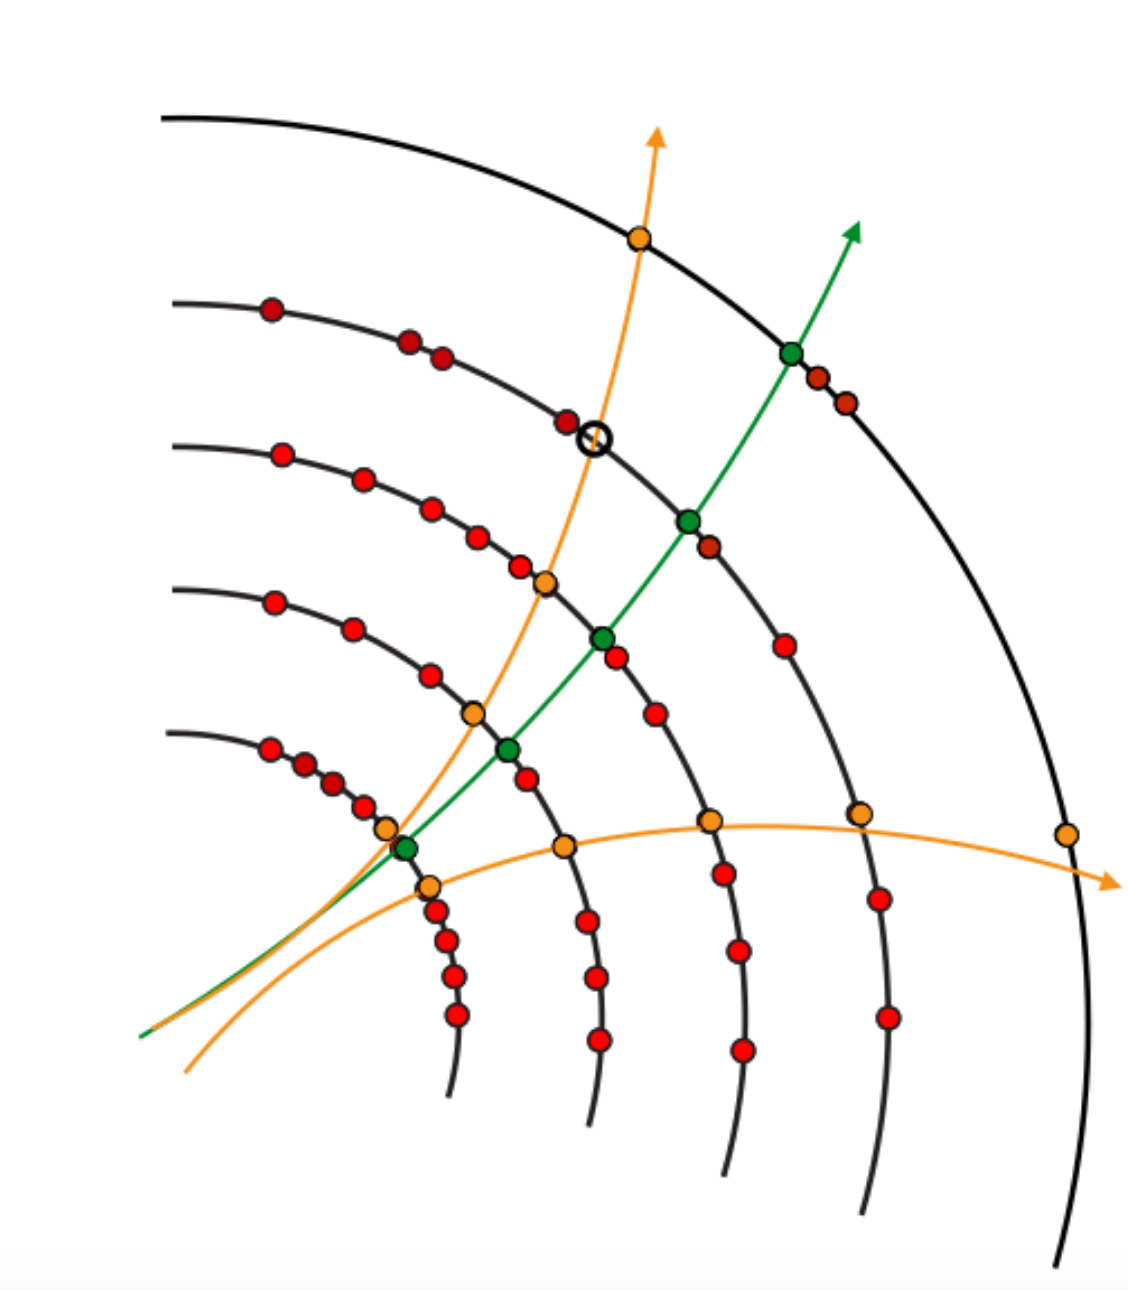
\includegraphics[width=0.30\textwidth]{./plots/TrackReconstruction.png}
\caption{Reconstructing one track from hits in a general-purpose detector. In green a good reconstruction, in orange two bad reconstructions~\cite{TrackMLPPTBefore}.}
\label{fig:FromHitsToTracks}
\end{figure}

\begin{figure}[!htb]
\centering
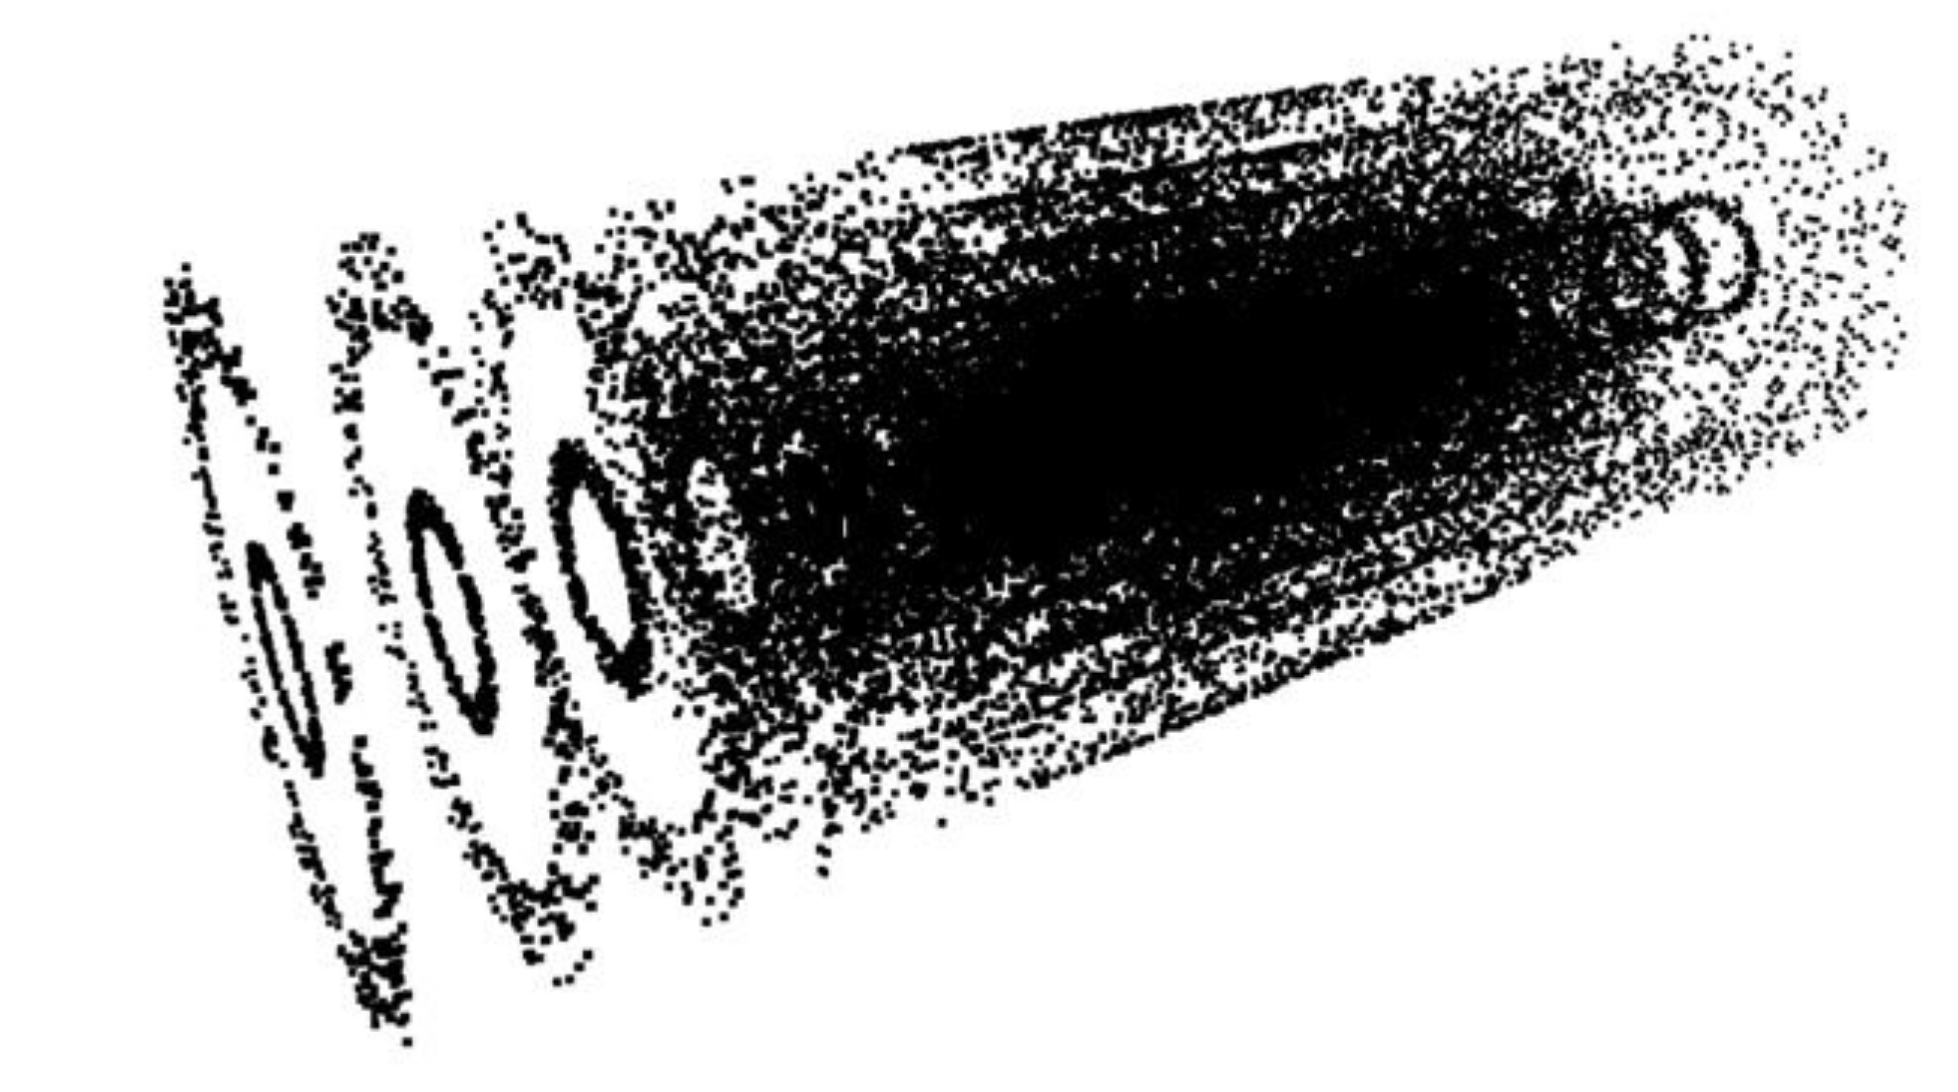
\includegraphics[width=0.49\textwidth]{./plots/Hits.png}
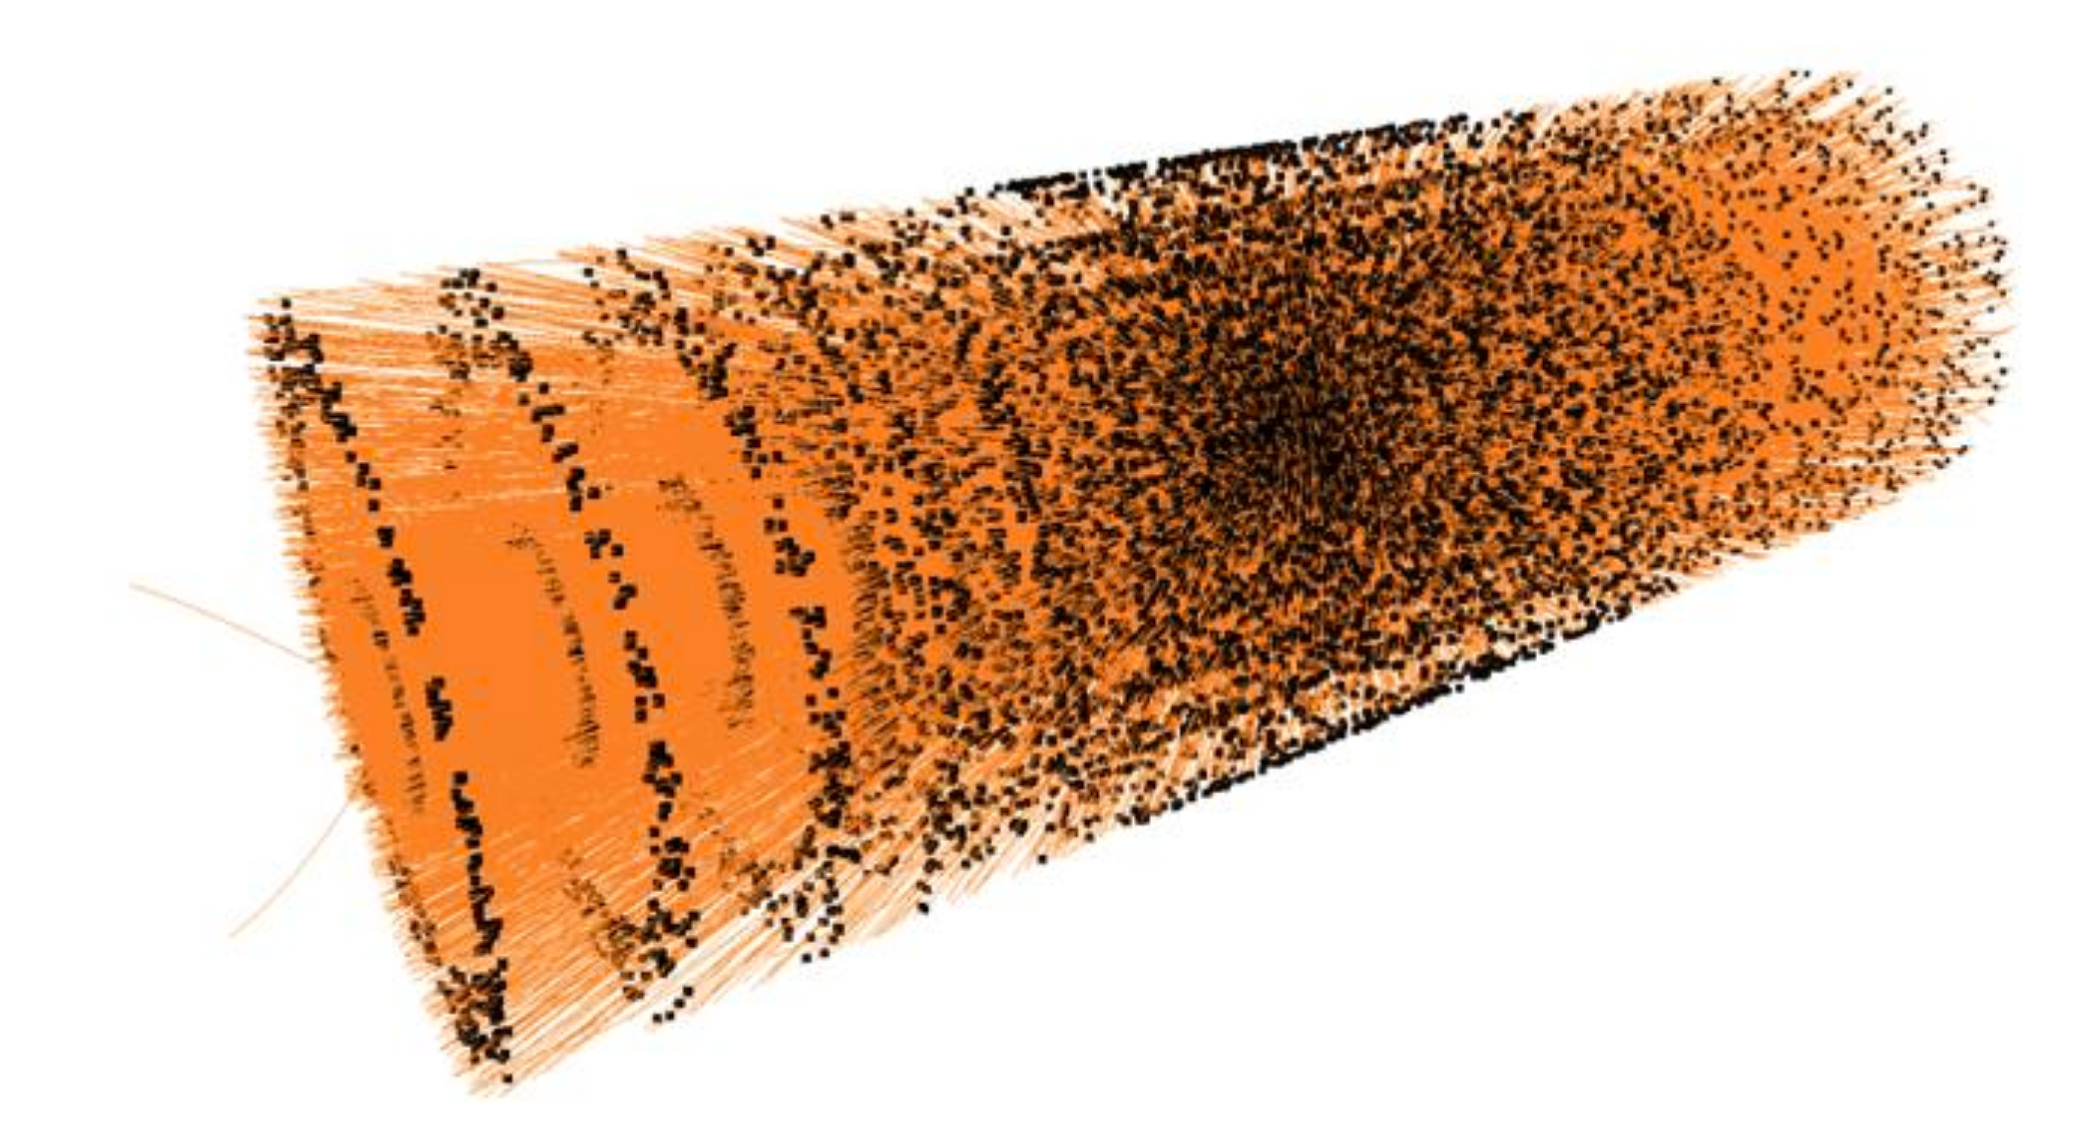
\includegraphics[width=0.49\textwidth]{./plots/Tracks.png}
\caption{Tracking for a general-purpose detector illustrated by reconstructing tracks (orange lines to the right) from hits (black individual 3D points to the left)~\cite{TrackMLPPTAfter}~\cite{TrackMLPPTAfter2}.}
\label{fig:FromHitsToTracks2}
\end{figure}

\ \\Tracking is a key component of event reconstruction and is used in several of its steps. The first step is to reconstruct vertices. Every proton collision in a bunch-crossing produces its own particles, out of which only the charged particles produce tracks. These tracks are clustered in a vertex. From the vertices in an event, the most interesting one (usually at higher energy for a rare particle) is called the \emph{primary vertex}, the rest being \emph{pile-up vertices}, as illustrated in Figure~\ref{fig:Vertices} for the ATLAS detector. 

\begin{figure}[!htb]
  \centering
  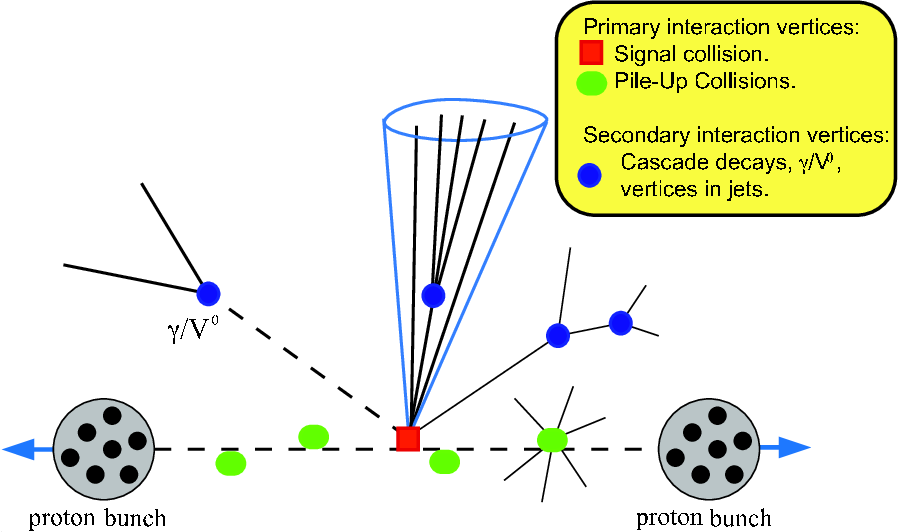
\includegraphics[width=0.45\textwidth]{plots/Vertices.png} 
  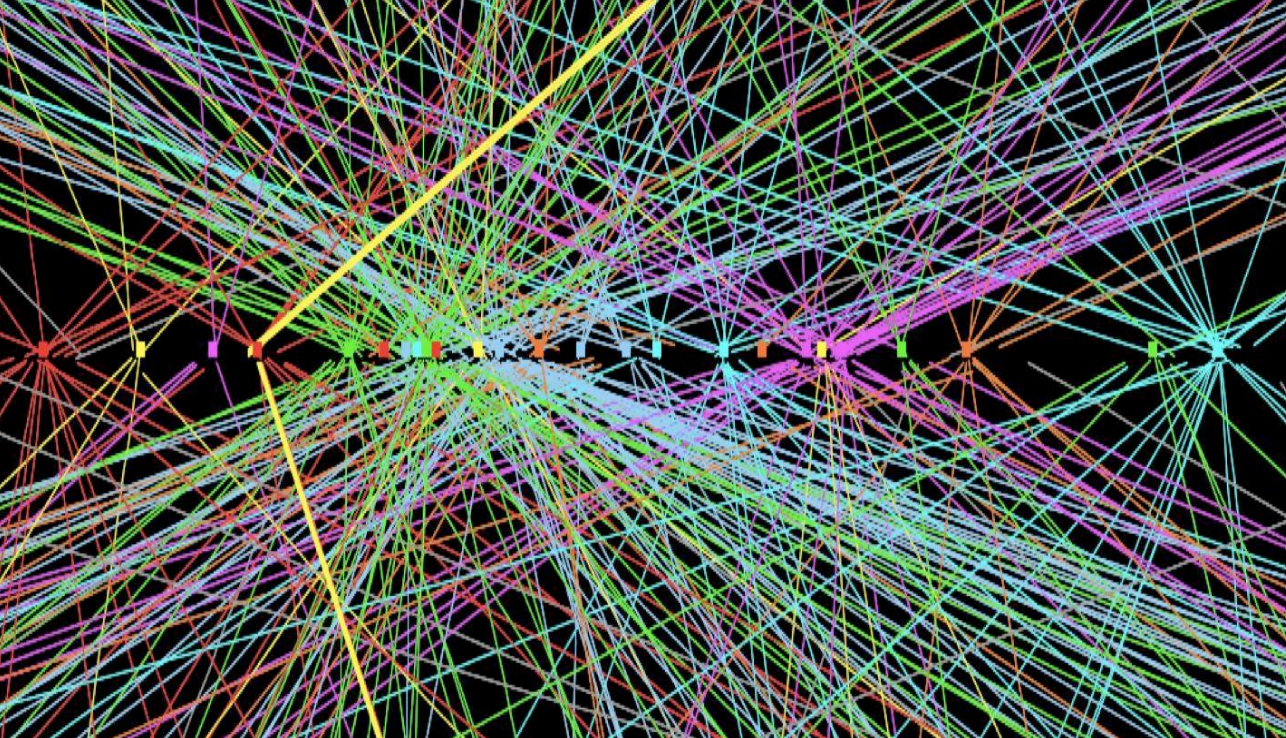
\includegraphics[width=0.45\textwidth]{plots/Vertices2.png} 
  \caption{Left: Diagram of the collision of proton bunches producing several vertices: one primary vertex from a rare interesting particle, and several pile-up vertices~\cite{ATLASVertices}. Right: Example of several vertices reconstructed in the ATLAS detector~\cite{TrackMLPPTBefore}.}
  \label{fig:Vertices}
\end{figure}

\ \\The second step is to reconstruct charged particle tracks. For example, an electron is reconstructed as a track in the ID, plus an electromagnetic shower in the EMCal. A muon is reconstructed as a track in the ID, plus energy deposits in the muon detector. A charged hadron is reconstructed as a track in the ID, plus a hadronic shower in HadCal. 

%\ \\Tracking is also key to reconstruct bottom ($b$) quarks. Top quarks decay about 100\% of the time into a $W$ boson and a $b$ quark. The Higgs boson decays most often (about 60\% of the time) to bottom-quark pairs. Also many supersymmetric particle decay signatures contain a $b$ quark. Identifying jets originating from bottom quarks is called \emph{b-tagging}. $b$-tagging uses tracks originating from the same vertex to identify a secondary vertex produced by the $B$-hadron decay after it has travelled about 3 mm away from the primary vertex.

\ \\Current tracking algorithms employed at ATLAS~\cite{TrackingATLAS} and CMS~\cite{TrackingCMS} use a combinatorial approach. First a track seed is found and later the track is computed. These algorithms require many calculations and thus require high CPU consumption. There is a stringent need to find algorithms with reduced CPU consumption to allow scaling from an LHC pile-up of about $\mu=36$ in Run-2 to $\mu=200$ in Run-3 and beyond. As illustrated in Figure~\ref{fig:CPU} (left), the CPU consumption increases more than quadratically with $\mu$. Tracking represents the largest part of the event reconstruction CPU. Figure~\ref{fig:CPU} (right) illustrates how the CPU consumption increases even further for Run-4 and Run-5. Especially for Run-4, scheduled for 2026, significant algorithm improvements are needed to improve tracking CPU requirements by a factor of approximately 10~\cite{TrackMLPPTBefore}.

%The CPU requirement increases further with increasing pile-up ($\mu$), due to the increased number of combinations of hits. Alternative more efficient algorithms are needed. In this thesis a machine learning algorithm is studied to reconstruct tracks at $\mu=200$ for the Run-3 through Run-5 at the LHC, using simulated data from the Particle Tracking Machine Learning Challenge, described in Chapter~\ref{chapter:TrackML}.

\begin{figure}[htb]
\centering
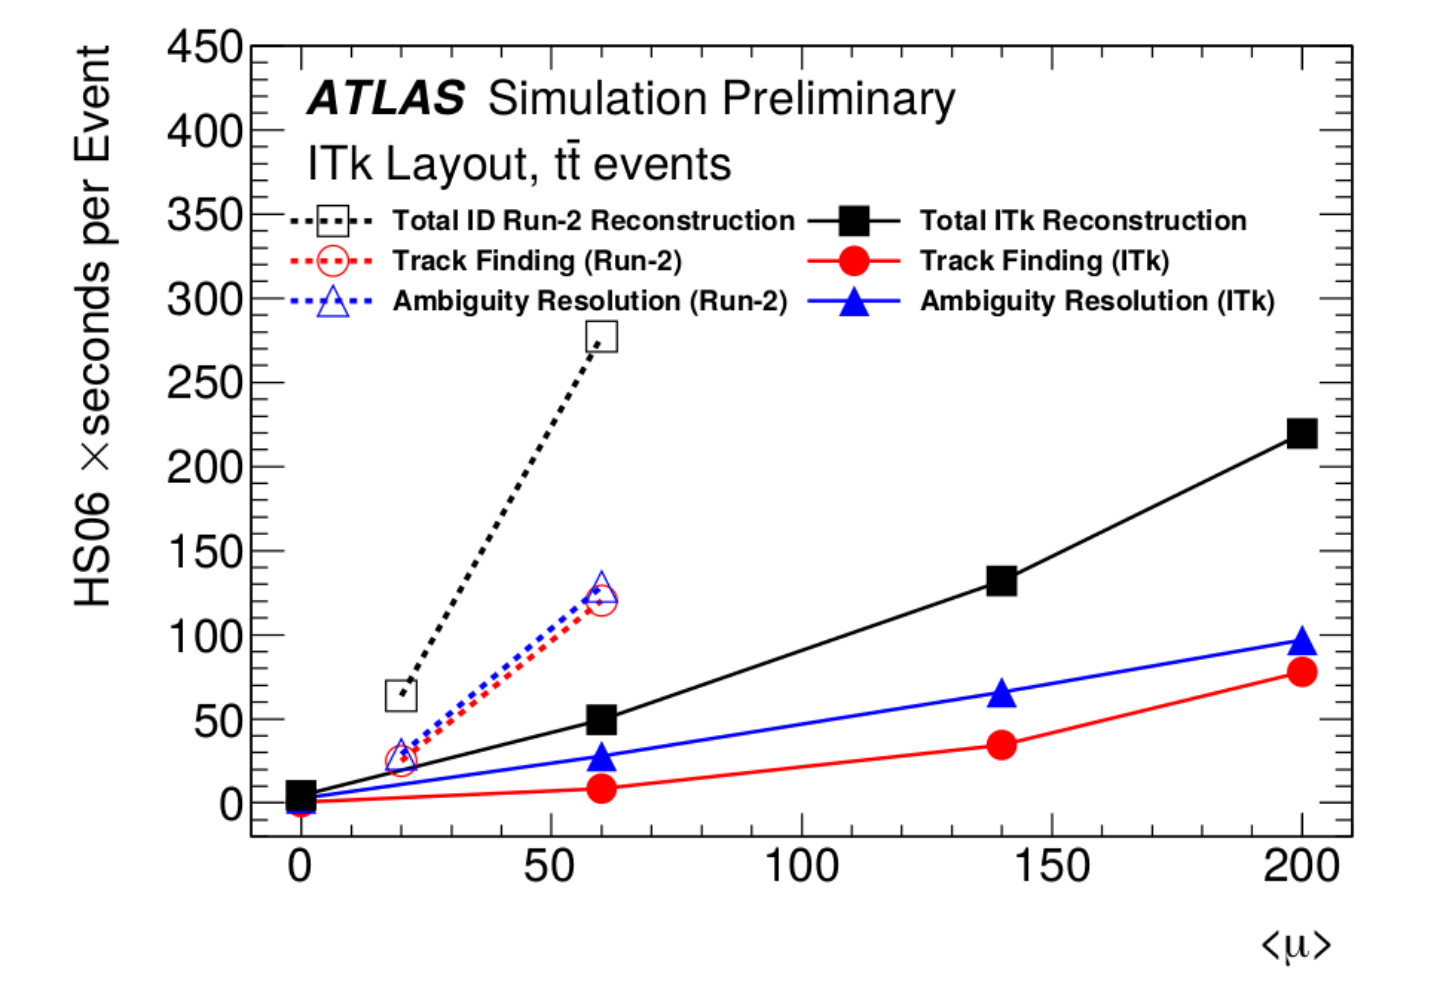
\includegraphics[width=0.45\textwidth]{./plots/CPU1.png}
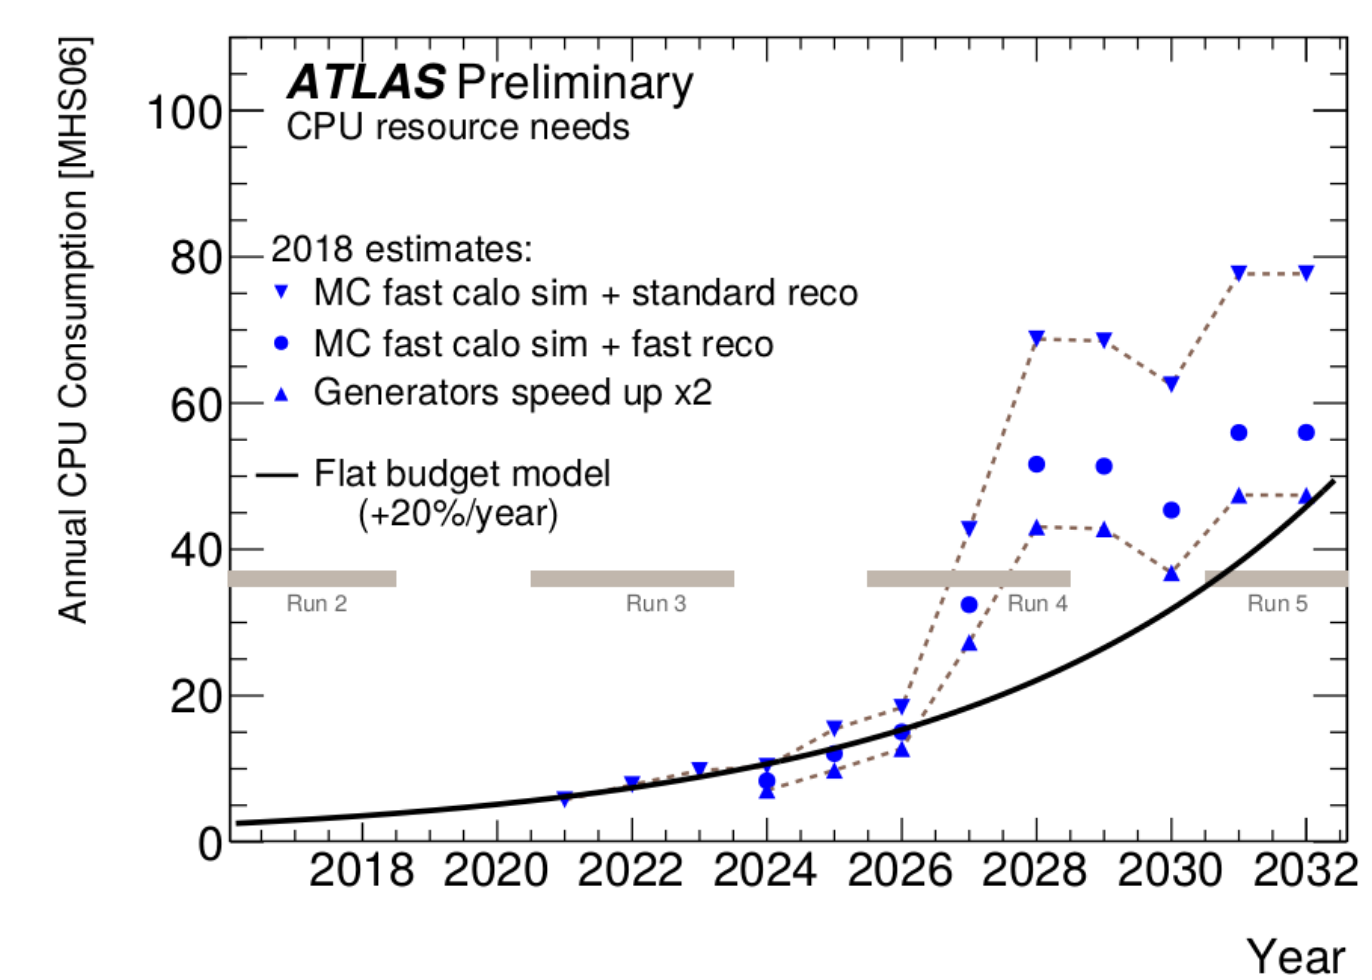
\includegraphics[width=0.45\textwidth]{./plots/CPU2.png}
\caption{CPU consumption increases more than quadratically with both pile-up (left) and years (right)~\cite{TrackMLPPTAfter}~\cite{TrackMLPPTAfter2}.}
\label{fig:CPU}
\end{figure}

\ \\A promising avenue is machine learning algorithms. Such algorithms require a lot of training data and require a long time to train (learn), but are usually fast to predict (infer). The field of machine learning has experienced a rapid growth in last few years. In this thesis a deep neural network algorithm is studied.
